\section{Semtools Framework}
\label{sec:framework}

The Semtools project has focused development efforts on three main
components: a Java library for accessing and manipulating OBOE
ontology extensions and semantic annotations, an annotation plugin for
the Morpho metadata editor, and query extensions for the Metacat data
catalog. Below we briefly describe these components and give a brief
overview of the OBOE model as well as the semantic
annotation approach used in Semtools. For a more in-depth presentation of OBOE see
\cite{madin07:_ontol_for_descr_and_synth,bowers08}.


\mypara{The OBOE Observational Model.}  \figref{fig:oboe} shows the
main modeling constructs of OBOE (see:
\url{http://ecoinformatics.org/oboe/oboe.1.0/oboe-core.owl}). An {\em
  observation} is made of an {\em entity} (e.g., biological organisms,
geographic locations, environmental features) and serves to group a
set of measurements together to form a single ``\emph{observation
  event}''. A \emph{measurement} assigns a value to a {\em
  characteristic} of the observed entity (e.g., the weight of a
plant), and can also include \emph{standards} (e.g., units as well as
standards for coded values) and collection \emph{protocols}. An
observation can occur within the surrounding \emph{context} of other
observations (e.g., as part of a temporal or spatial context), and
context may include a named relationship (e.g., ``partOf'',
``within'') that existed during the observation event. A key feature
of OBOE is that it allows properties (characteristics and
relationships) of entities to be asserted without being interpreted as
\emph{inherently} (i.e., {always}) true of the entity.  Depending on
the context in which the entity was observed or how the measurements
were performed, an entity's properties may take on different values.
OBOE allows RDF-style assertions about entities to be contextualized,
and thus different values can be assigned for the same entity under
distinct contexts, which is a crucial feature for modeling ecological
as well as many other types of scientific data
\cite{bowers08,mungall07:_repres_phenot_in_owl}. In addition, OBOE is
currently implemented as an OWL-DL ontology that can be easily used
with (or extended by) other ontologies for specifying domain-specific
types of entities, characteristics, measurement standards, protocols,
and relationships. For instance, the Semtools project has defined
specific OBOE extensions in collaboration with the Santa Barbara
Coastal Long-Term Ecological Research Project as well as through
ongoing collaborations with other projects, and general extensions
exist for OBOE that define a number of common entities, measurement
units, and corresponding physical characteristics.

\begin{figure}[!t]
  \centering
  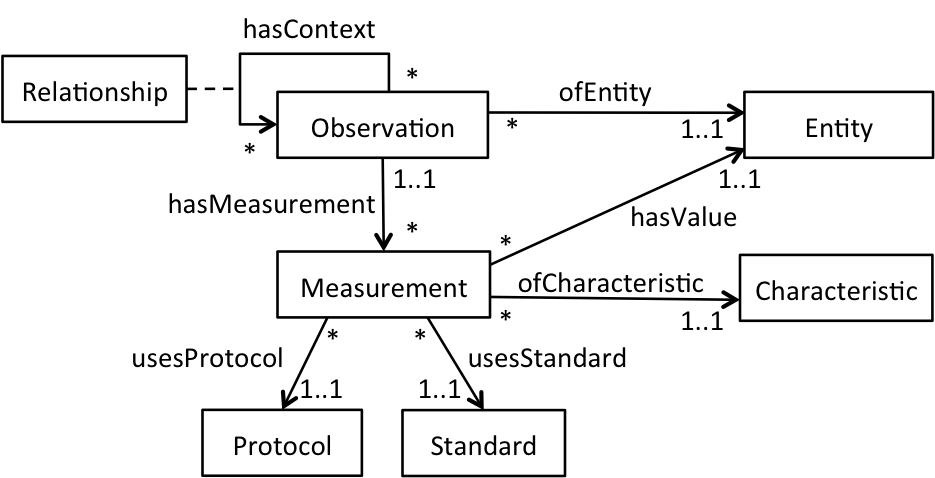
\includegraphics[width=0.49\textwidth]{images/oboe}
  \caption{The main classes and properties of the extensible
    observation ontology (OBOE). While shown using UML, the model is
    defined using OWL-DL.}
  \label{fig:oboe}
\end{figure}

\mypara{Semantic Annotations.} A semantic annotation consists of two
parts: (i) a ``configuration'' of the observation model containing the
specific entities, characteristics, observations, measurements, and so
on (drawn from one or more domain ontologies) that appropriately
capture the semantics of the data set; and (ii) a mapping between the
attributes in the data set to specific measurements defined in the
model configuration. \figref{fig:kelp-mass-model} shows a high-level
example of an annotation defined for a simple Kelp sampling data
set. Here, the data set consists of five attributes (bottom of
\figref{fig:kelp-mass-model}). Each attribute is mapped to a specific
measurement type (where only the characteristic of each measurement
type is shown), and measurement types are organized into observations
of specific Kelp entities (shown of type ``Macrocystis''), temporal
points (denoted by date-times), and spatial locations (given as site
names). Each measurement associated with a Kelp observation is assumed
to have occurred within the site and during the given time as
specified by the context relationships.  Semantic annotations provide
a formal description of attribute semantics, whereas in many
commonly-used metadata formats for describing data sets,  only
informal text-based descriptions of data attributes are permitted.  In
the case of EML, there is some overlap between these two
mechanisms---particularly with respect to measurement
standards---however, semantic annotations extend this approach by
providing a general mechanism to formally associate concepts drawn
from domain ontologies to attributes. In the Semtools framework, we
employ an XML serialization syntax for semantic annotations that is
compatible with EML but that is stored separately from the EML
documentation of a data set (allowing, e.g., annotations to be used
independently of EML or with other metadata standards if needed). In addition, semantic annotations can
be used to ``materialize'' a given data set into a set of triples
conforming to the model configuration given in the annotation.
Materializing a data set to a set of OBOE triples in this way provides
a more uniform structural representation that can make a number of
integration tasks easier (described further below).

% Because the Annotation represents a potentially subjective
% perspective on the data, they are stored independently as XML; the
% former referencing the latter.  The Annotation structure largely
% mirrors the core classes in OBOE. Observations are composed of
% Measurements of a specific Entity and are represented by a
% collection of Characteristics (usually just one) collected using a
% defined Protocol and Standard (i.e. unit).  Tablular data object
% attributes are mapped to a Measurement such that a collection of
% attributes usually pertain to the Entity of a shared Observation
% (\figref{fig:kelp-mass-model}). These Observtions can provide
% context for other Observations such that the structure of the
% observational data model and collection paradigm are formally
% represented in the Annotation.


\begin{figure}[!b]
\centering
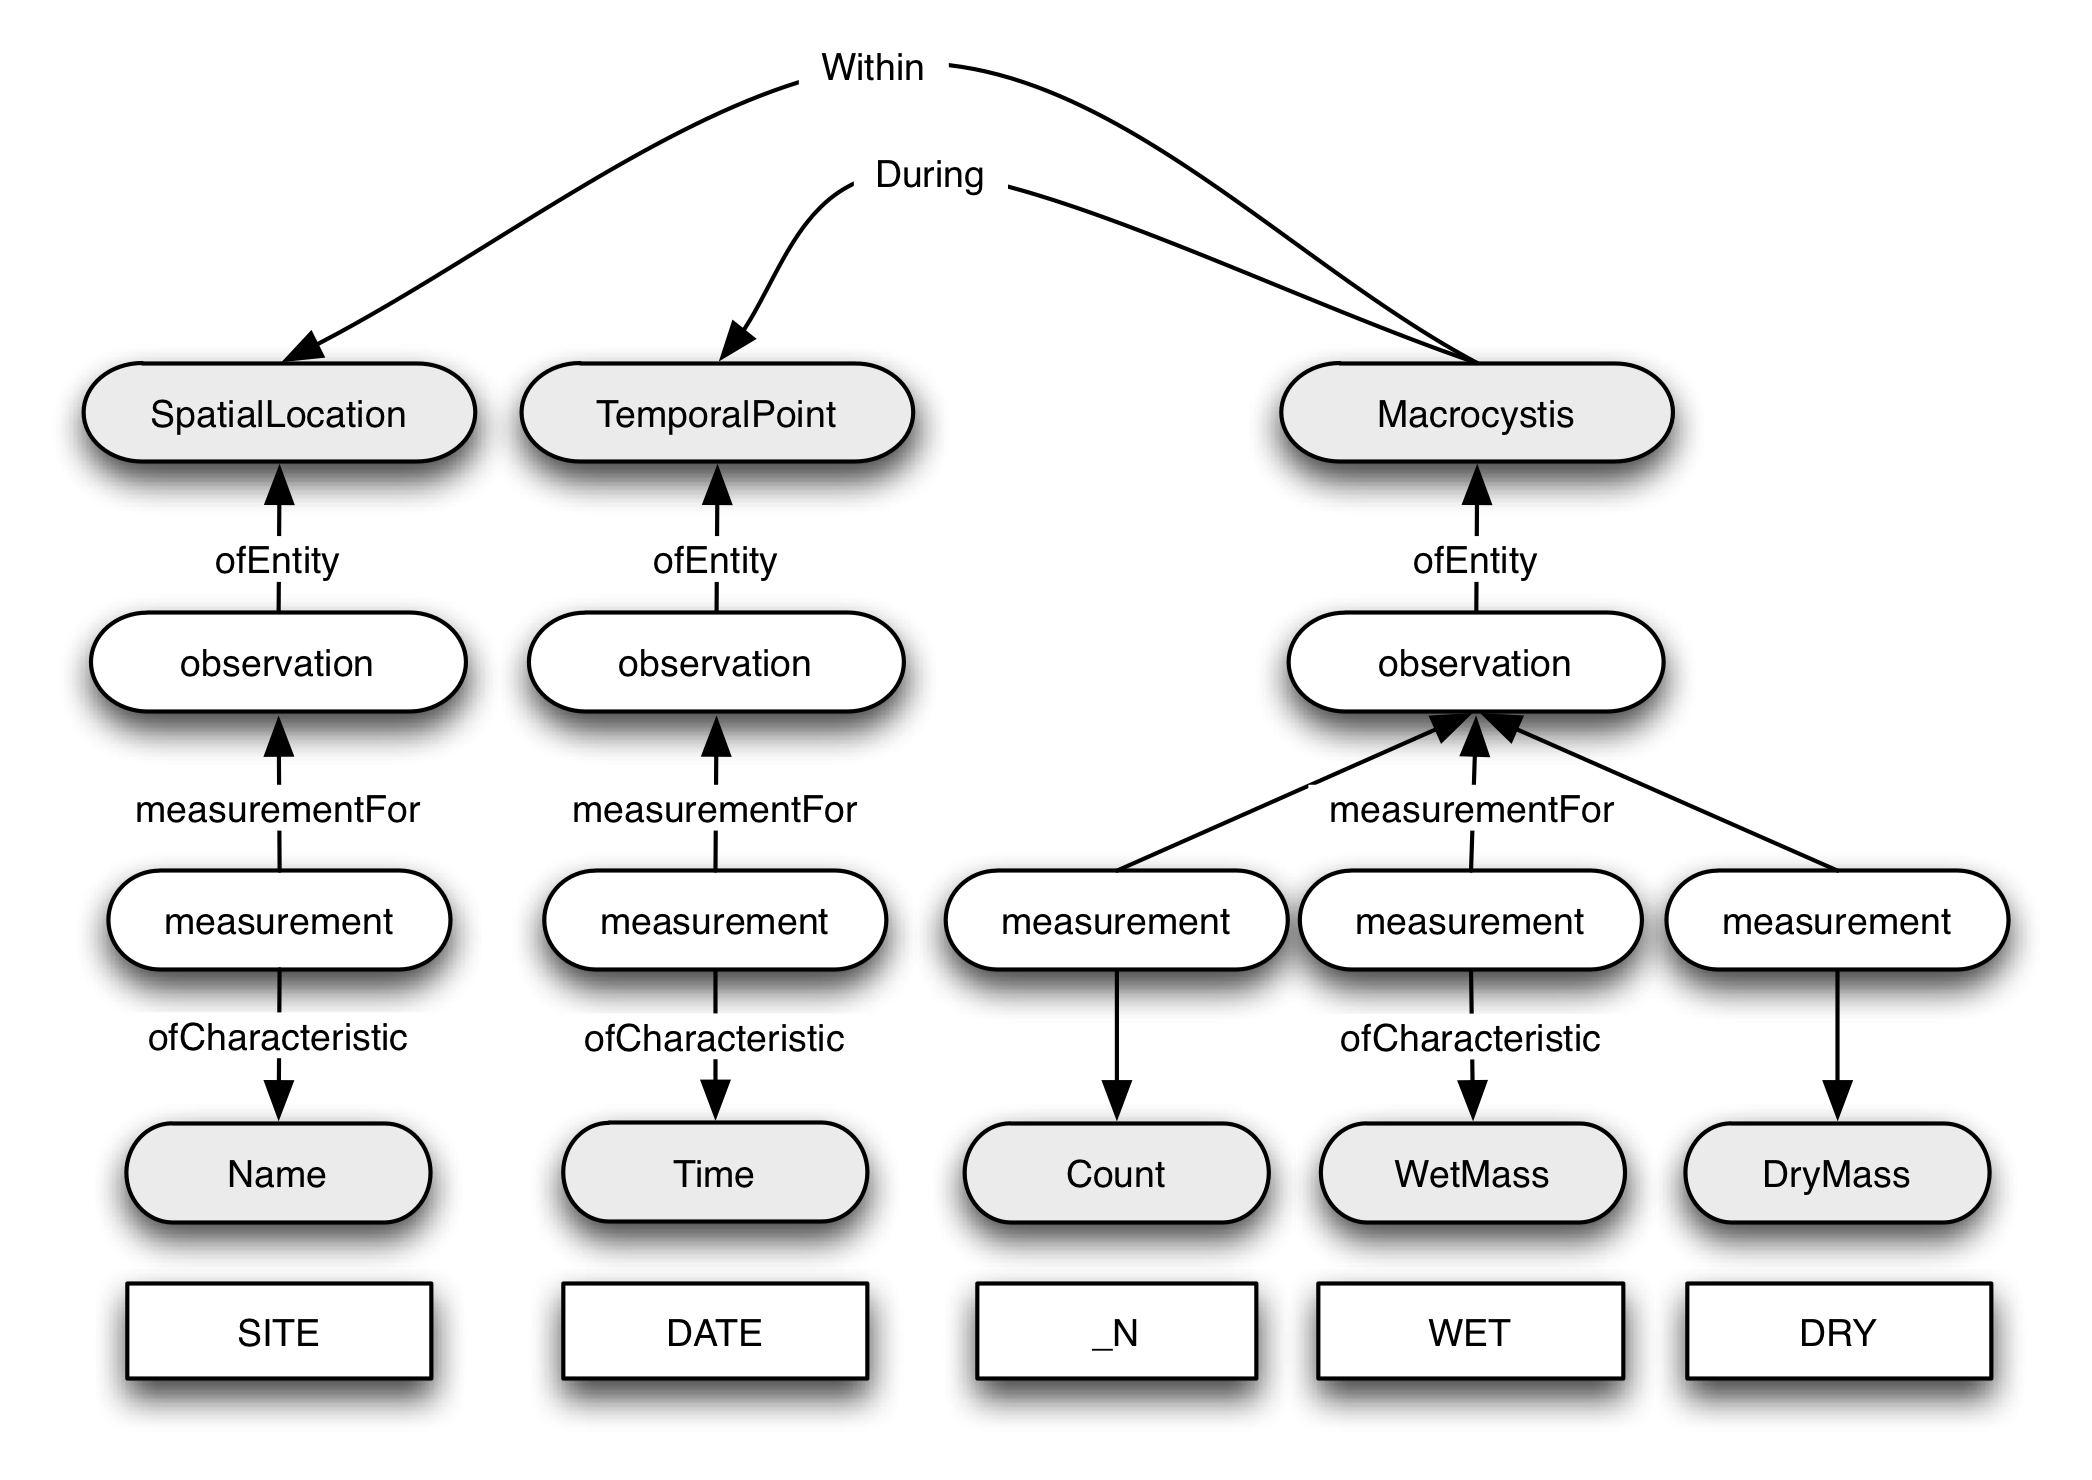
\includegraphics[width=0.5\textwidth]{images/kelp-mass-model.png}
\caption{Partial OBOE semantic annotation for Kelp sampling
  data. Shaded nodes represent ontological concepts; rectangular nodes
  are data table attibutes mapped to OBOE measurement
  characteristics.}
\label{fig:kelp-mass-model}
\end{figure}

\begin{figure*}[!t]
\centering
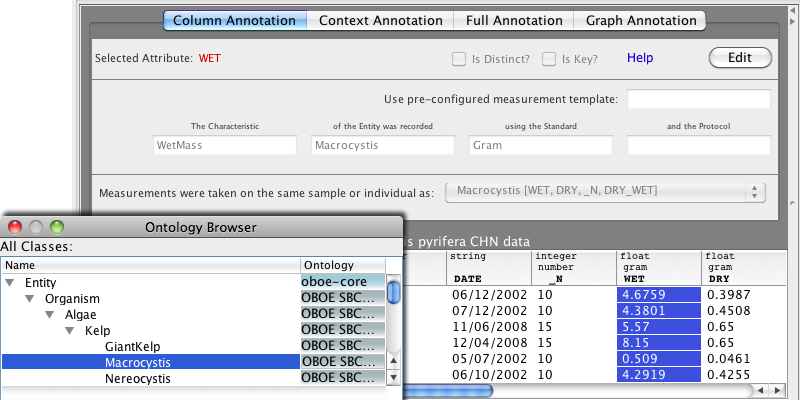
\includegraphics[width=1.0\textwidth]{images/morpho-annotation-widget.png}
\caption{Morpho metadata editor with Semantic
  plugin. The fill-in-the-blank interface uses
  natural language descriptions for intuitive editing. A searchable, hierarchical browser is
  used to select concepts from domain-specific ontologies.}
\label{fig:morpho-annotation}
\end{figure*}

\mypara{The Semantic Mediation API.} The Semantic Mediation API
includes basic ontology management features, annotation manipulation
capabilities, and simple concept navigation and visualization
components. The API is intended to be a centralized toolkit for use in
multiple application contexts (on either client or server deployments).
The Semantic Mediation API uses both the OWL API \cite{owlapi} for ontology
management services including RDF/OWL parsing, serialization, and
simple class and property exploration as well as the Pellet
description-logic reasoner \cite{pellet} for classification and exposing
inferred axioms in source ontologies. The inference services exposed
through the Semantic Mediation API are used in both discovery and
integration described below.
% is particularly powerful when utilizing OBOE Measurement 'templates'
% that express exactly what (Entity and Characteristic) can be
% observed and how (Standard and Protocol).
In our current Morpho and Metacat extensions, semantic annotations are
managed and stored automatically in an underlying, local relational
database. While it is also possible to use in-memory approaches for
storing and querying annotations, we found the overhead to be
prohibitive when large numbers of data sets are managed.

% store and query annotations inmemory
% approachesfor storing for scalable persistence and improved query
% performance, which we found to be essential when large numbers of data
% sets are supported. , where the overhead of in-memory annotation
% queries having proven to be prohibitively limiting for large sets of
% data.



\mypara{The Morpho Editor Plugin.}  The semantic-annotation editor
plugin for Morpho provides a front-end to the Semantic Mediation API
and allows users to define annotations for existing data package
descriptions. The editor provides a simple ``fill-in-the-blank'' style
form-based interface with a searchable hierachical concept selection
widget (see \figref{fig:morpho-annotation}). The plugin seamlessly
integrates with a standard Morpho installation and provides semantic
query capabilities for locating data packages, marking up data
packages with semantic annotations, and saving annotations locally or
to a shared repository where they can be discovered and explored by
other users. The annotation editor in Morpho allows a user to view the
data set being annotated and fill in (by selecting an appropriate
ontology term) the characteristic, measurement standard, protocol, and
associated entity for each data-set attribute. Users can also specify
whether an observation spans multiple columns, and can provide context
relationships between attributes (i.e., obserations). The editor
provides a number of additional features including allowing users to
view the entire annotation (similar to \figref{fig:kelp-mass-model})
and to specify additional mapping constraints for observations and
measurements.

\mypara{Metacat Query Extensions.}  The semantic plugin for Metacat
augements Metacat's existing metadata storage and search by allowing
annotations to be saved and queried alongside the metadata and data
that they annotate. In addition to traditional keyword and spatial
search criteria, the Metacat plugin allows semantic criteria to be
included where they may either increase query recall using
term-expansion (i.e., traversing the class subsumption hierarchy) or
refine the resultset by limiting matches to datasets that contain the
specified observational model (e.g., combinations of OBOE-compatible
entity, characteristic, measurement standard, or protocol
concepts). The observational model can be leveraged further by
materializing the annotation and data artifact (via the Data Manager
Library \cite{leinfelder10:_metad_driven_approac_to_loadin}) into a
fully instantiated OBOE model and inspecting (and querying over) the
observational values themselves.

%%% Local Variables: 
%%% mode: latex
%%% TeX-master: "main"
%%% End: 
